\section{Token Balancing and Response Length}
\label{sec:normalization}

\subsection{How does loss averaging change domain weights?}

The response-normalized objective in Equation~\ref{eq:mopd} gives each response equal weight within its domain. Averaging all valid tokens together instead makes response length part of the weighting rule. Open-MOPD identifies this effect under token-mean aggregation \citep[Section~3.3]{gao2026openmopddiagnosingfixingcapability}. Separating domain weights from response weights makes the effect of each averaging rule explicit.

For response $i$, let $T_i$ be its valid-token count and $\ell_i=T_i^{-1}\sum_t\ell_{i,t}$ its mean token loss. Let $\mathcal B_d$ contain the responses from domain $d$, with target weights $\sum_d\lambda_d=1$. Table~\ref{tab:normalization} compares the three reductions on the same batch.

\begin{table}[t]
\caption{Averaging rules on a fixed batch of nonempty responses. GT assigns domains their observed token shares; DT fixes domain weights; DR also gives responses equal weight within each domain.}
\label{tab:normalization}
\centering\small
\renewcommand{\arraystretch}{1.2}
\begin{tabular*}{\linewidth}{@{\extracolsep{\fill}}ll@{}}
\toprule
Reduction & Batch loss \\
\midrule
Global token (GT) & $\sum_i T_i\ell_i/\sum_i T_i$ \\
Domain token (DT) & $\sum_d\lambda_d\,\sum_{i\in\mathcal B_d}T_i\ell_i/\sum_{i\in\mathcal B_d}T_i$ \\
Domain response (DR) & $\sum_d\lambda_d\,|\mathcal B_d|^{-1}\sum_{i\in\mathcal B_d}\ell_i$ \\
\bottomrule
\end{tabular*}
\end{table}

With equal prompt quotas, longer responses increase a domain's weight under GT. DT removes this between-domain length effect, while retaining length weighting within each domain. Writing $g_i=\nabla_\theta\ell_i$, the exact fixed-batch relation is
\begin{equation}
\frac{\sum_{i\in\mathcal B_d}T_i g_i}{\sum_{i\in\mathcal B_d}T_i}
=\bar g_d+\frac{\operatorname{Cov}_d(T,g)}{\bar T_d}.
\label{eq:weighting}
\end{equation}
Here $\bar g_d$ and $\bar T_d$ are domain averages, and the covariance measures whether longer responses contribute systematically different gradients. DT retains this covariance term; DR removes it. Moreover, multiplying GT terms by the target domain weight divided by the observed token share gives DT exactly. This is the token-share correction in Open-MOPD \citep[Section~4.1, Eq.~(8)]{gao2026openmopddiagnosingfixingcapability}. DR makes the additional choice of weighting responses equally within each domain. Appendix~\ref{app:normalization} gives the derivation.

\subsection{Experiment: averaging rules and capability balance}

\paragraph{Comparison.}
We train a Qwen3-1.7B student with four RL-trained teachers specializing in mathematics, code, instruction following, and science. The three branches use the same student/teacher top-64 intersection loss (I64; Appendix~\ref{app:losses}) and differ in global-token (GT), domain-token (DT), or domain-response (DR) averaging. They share initialization, teachers, prompt schedule, optimizer settings, and response cap. Each update uses 16 prompts per domain; DT and DR use domain weights $1/4$. Responses are sampled from each branch's current student. We compare all three branches at update 50 on four held-out benchmarks. Appendix~\ref{app:setup} gives the shared protocol and scoring.

\paragraph{Response length changes the loss weights.}
Across the first 50 GT rollout batches, mathematics receives a mean 44.05\% of valid tokens and instruction following 14.98\%, although each receives 25\% of prompts. Under GT, these are also their mean loss weights; DT and DR assign each domain 25\%. The mean mathematics weight is therefore nearly three times the mean instruction-following weight. Figure~\ref{fig:all_token_shares} gives the three branches' token shares over the same interval.

\begin{figure}[t]
\centering
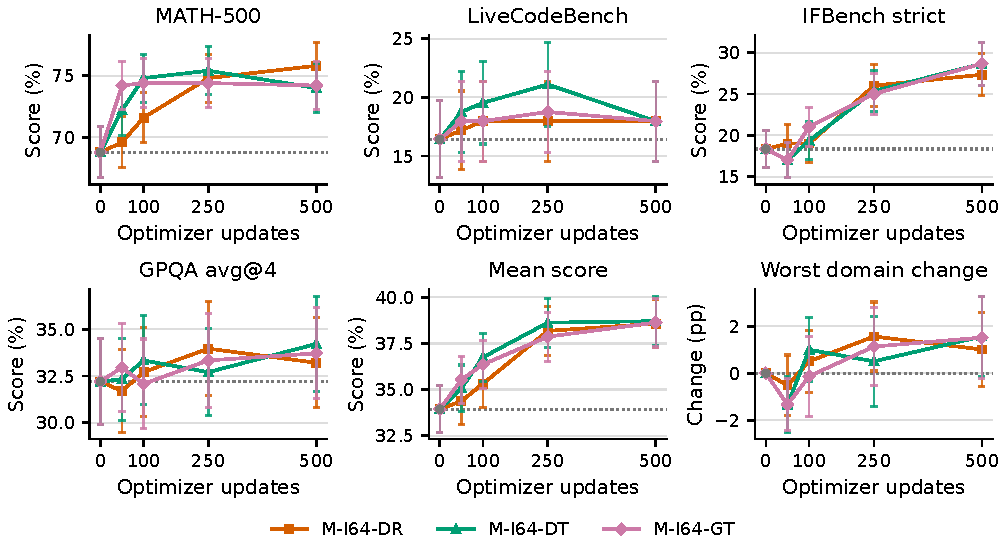
\includegraphics[width=\linewidth]{figures/aligned_evidence_20260910/normalization_capability.pdf}
\caption{GT/DT/DR capability comparison at update 50. The first four panels show domain scores, followed by their arithmetic mean and the smallest domain change from initialization. The initial student is shared. Lines connect the initial and update-50 evaluations; all three branches use one common training seed.}
\label{fig:normalization_capability}
\end{figure}

\paragraph{Within-domain length weighting changes the gradient.}
We also hold the student and response batch fixed, then recompute I64 gradients under all three reductions. The comparison uses M-PG checkpoints 100 and 250, each with three banks of eight responses per domain. DT and DR have the same domain weights, yet the cosine between their raw gradients ranges from 0.578 to 0.911 at update 100 and from 0.399 to 0.786 at update 250. Thus response weighting changes gradient direction even after the domain weights are fixed. Table~\ref{tab:fixed_batch_normalization} reports all six banks and all three pairwise comparisons. This isolates the within-batch weighting effect in Equation~\ref{eq:weighting}; the online branches above include the evolution of student-generated responses.

\paragraph{Averaging redistributes capability gains.}
GT achieves 74.2\% on mathematics versus DR's 69.6\%, a difference of 4.6 percentage points with a paired prompt-bootstrap interval of $[1.2,8.2]$. DR achieves 19.0\% on instruction following versus 17.0\% for both GT and DT. The DT-minus-DR interval on instruction following is $[-4.0,-0.33]$ points. Thus the rule with the highest mathematics score has a lower instruction-following score, while equal domain weights in DT still produce a different tradeoff from equal response weights in DR. Figure~\ref{fig:normalization_ci} reports all eight domain-level contrasts.

Table~\ref{tab:normalization50} gives the score comparison. GT has the highest four-domain mean (35.53\%), while DR has the smallest decline on its most affected domain ($-0.51$ points, compared with $-1.33$ for DT and GT). These summaries express two different goals: average capability and preserving capability across domains. The length-weighting identity explains which training examples receive more weight; the measured scores determine the resulting tradeoff.

\begin{table}[t]
\caption{Capability scores (\%) at update 50. Mean averages the four domain scores. Worst $\Delta$ is the smallest domain change from initialization, in percentage points.}
\label{tab:normalization50}
\centering\small
\begin{tabular}{lrrrrrr}
\toprule
Reduction & Math & Code & IF & GPQA & Mean & Worst $\Delta$ \\
\midrule
DR & 75.80 & 17.97 & 27.33 & 33.21 & 38.58 & +1.01 \\
DT & 74.00 & 17.97 & 28.67 & 34.22 & 38.71 & +1.56 \\
GT & 74.20 & 17.97 & 28.67 & 33.71 & 38.64 & +1.52 \\
\bottomrule
\end{tabular}

\end{table}

\completionnote{Later-checkpoint normalization comparison}{Complete the GT, DT, and DR capability evaluations at a common later checkpoint before adding its comparison figure or table. The update-50 comparison above contains all three branches.}
